\newpage
\definecolor{lblue}{rgb}{0.39, 0.58, 0.93}
%\blfootnote{\color{toancuabi}$^1$Đại học Thăng Long.}
%\everymath{\color{toancuabi}}
\graphicspath{{../timhieucungbi/demtamgiac2/}}

Các bạn nhỏ ơi, chúng ta đã đi gần hết chặng đường rồi. Dưới đây là nhiệm vụ cuối cùng. Nhiệm vụ cuối nên sẽ khó hơn một chút. Chúng ta cùng nhau tìm ra “câu thần chú” nhé. 
\vskip 0.1cm
{\bf\color{toancuabi} Bài toán $\pmb{4.}$ Đếm số tam giác với hoa văn đặc biệt kiểu tam giác}
\vskip 0.1cm
{\bf\color{toancuabi} Ví dụ $\pmb{4.}$} Các hình sau có bao nhiêu tam giác?
	\begin{figure}[H]
	\centering
	\vspace*{-5pt}
	\captionsetup{labelformat= empty, justification=centering}
	\captionsetup[subfigure]{labelformat=empty}
	\hfill\subfloat[\textit{\color{toancuabi}Hình} $17.$]{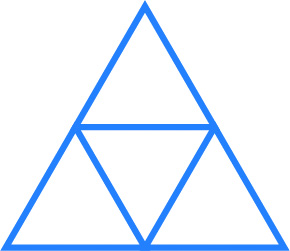
\includegraphics[width=0.14\textwidth]  
		{Hinh23}}
	\hfill
	\subfloat[\textit{\color{toancuabi}Hình} $18.$]{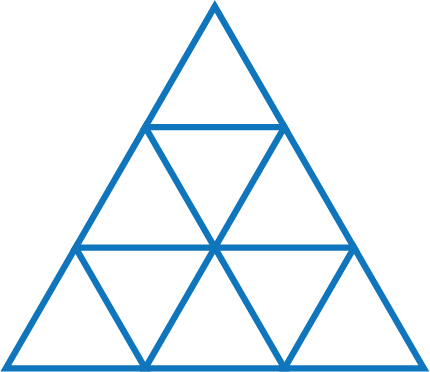
\includegraphics[width=0.19\textwidth]{Hinh24}}
	\hfill\subfloat[\textit{\color{toancuabi}Hình} $19.$]{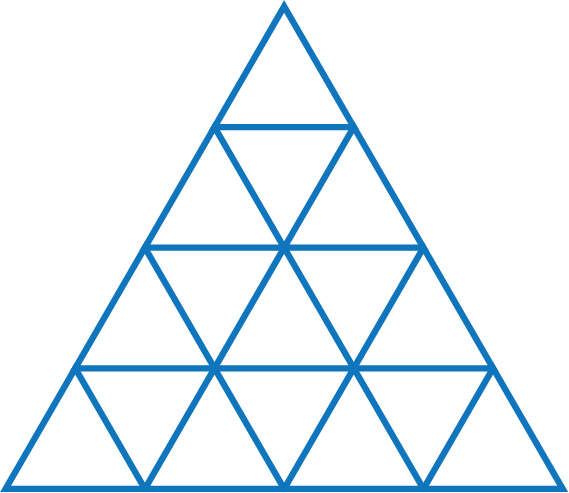
\includegraphics[width=0.25\textwidth]{Hinh25}}
	\hfill
	\vspace*{-10pt}
\end{figure}
{\bf\color{toancuabi} Lời giải.}
\vskip 0.1cm
Ở đây để tiện cho việc ký hiệu, ta quy ước mỗi tam giác đơn có cạnh kích thước $1$ (đơn vị).
\vskip 0.1cm
Hình $17$ là tam giác với cạnh có kích thước $2$, chúng ta có thể dễ dàng thấy hình này có $5$ tam giác, trong đó có $4$ tam giác đơn và $1$ tam giác bốn.
\vskip 0.1cm
Hình $18$ là tam giác với cạnh kích thước $3$, không mấy khó khăn ta đếm được Hình $23$ có $13$ tam giác, trong đó có $9$ tam giác đơn, $3$ tam giác bốn và $1$ tam giác chín.
\vskip 0.1cm
Tuy nhiên, khi kích thước cạnh tăng lên là $4$ như Hình $19$ hay kích thước cạnh là $5$ hoặc nhiều hơn nữa thì việc đếm số tam giác trở nên phức tạp hơn nhiều. Do đó, ta phải nhanh chóng tìm ra ``câu thần chú" cho bài toán đếm tam giác dạng này nhé. 
	 \begin{figure}[H]
	\centering
	\vspace*{-5pt}
	\captionsetup{labelformat= empty, justification=centering}
	\captionsetup[subfigure]{labelformat=empty}
	\hfill\subfloat[\textit{\color{toancuabi}Tam giác hướng lên -- Kích thước $1$.}]{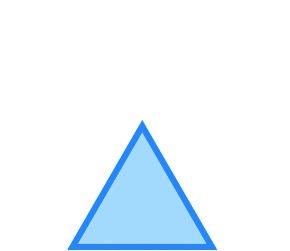
\includegraphics[width=0.19\textwidth]  
		{HinhHL11}}
	\hfill
	\subfloat[\textit{\color{toancuabi}Tam giác hướng lên -- Kích thước $2$.}]{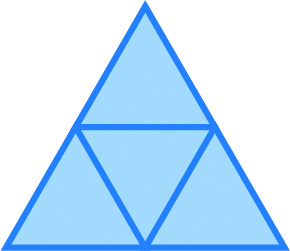
\includegraphics[width=0.19\textwidth]{HinhHL2}}
	\hfill
	\subfloat[\textit{\color{toancuabi}Tam giác hướng~xuống~-- Kích thước~$1$.}]{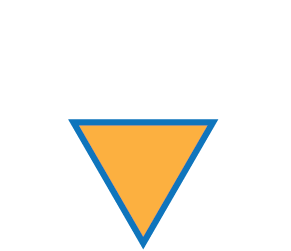
\includegraphics[width=0.19\textwidth]{HinhHX11}}
	\hfill
	\subfloat[\textit{\color{toancuabi}Tam giác hướng~xuống~-- Kích thước~$2$.}]{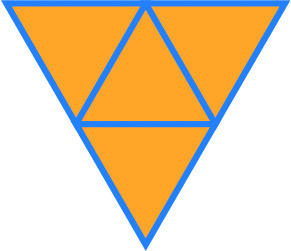
\includegraphics[width=0.19\textwidth]{HinhHX2}}
	\hfill
	\vspace*{-10pt}
\end{figure}
Với bài toán này, ta sẽ giới thiệu một kiểu đếm mới, đó là đếm theo số tam giác {\color{timhieukhoahoc}{``hướng lên"}} và {\color{duongvaotoanhoc}{``hướng xuống"}}.
\vskip 0.1cm
Ta nhận thấy số tam giác cần đếm bằng tổng số tam giác ``hướng lên” và ``hướng xuống" trong hình. Bây giờ, ta lập bảng đếm số tam giác ``hướng lên" và ``hướng xuống" trong Hình $17$, Hình $18$ và Hình $19$ nhé.
\begin{multicols}{2}
	\begin{table}[H]
		\setlength{\tabcolsep}{2pt}
		\renewcommand{\arraystretch}{1.3}
		\begin{tabular}{|c|c|c|c|}
			\hline
			Vị trí & {\color{timhieukhoahoc}{Lên}}  & {\color{duongvaotoanhoc}{Xuống}} & {\color{red}{Tổng}}\\
			\hline
			Kích thước $1$ & ${\color{timhieukhoahoc}{3}}$ &${\color{duongvaotoanhoc}{1}}$ & ${\color{red}{4}}$\\
			\hline
			Kích thước $2$ & ${\color{timhieukhoahoc}{1}}$ & ${\color{duongvaotoanhoc}{0}}$ & ${\color{red}{1}}$ \\
			\hline
		\end{tabular}
	\end{table}
	\begin{figure}[H]
		\vspace*{-5pt}
		\centering
		\captionsetup{labelformat= empty, justification=centering}
		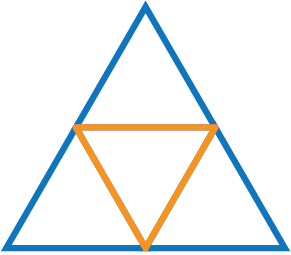
\includegraphics[width=0.125\textwidth]{Hinh23_1}
		\caption{\color{red}{\fbox{\small Tổng toàn bộ : $\color{red}4 + 1 = 5$}}}
		\vspace*{-5pt}
	\end{figure}
\end{multicols}
\begin{multicols}{2}
	\begin{table}[H]
		\setlength{\tabcolsep}{2pt}
		\renewcommand{\arraystretch}{1.3}
		\begin{tabular}{|c|c|c|c|}
			\hline
			Vị trí & {\color{timhieukhoahoc}{Lên}}  & {\color{duongvaotoanhoc}{Xuống}} & {\color{red}{Tổng}}\\
			\hline
			Kích thước $1$  & ${\color{timhieukhoahoc}{6}}$ &${\color{duongvaotoanhoc}{ 3}}$ &${\color{red}{9}}$ \\
			\hline
			Kích thước $2$  & ${\color{timhieukhoahoc}{3}}$ & ${\color{duongvaotoanhoc}{0}}$ & ${\color{red}{3}}$ \\
			\hline
			Kích thước $3$  & ${\color{timhieukhoahoc}{1}}$ & ${\color{duongvaotoanhoc}{0}}$ & ${\color{red}{1}}$ \\
			\hline
		\end{tabular}
		%		\caption{Bảng $1$.}
	\end{table}
	\begin{figure}[H]
		%			\vspace*{5pt}
		\centering
		\captionsetup{labelformat= empty, justification=centering}
		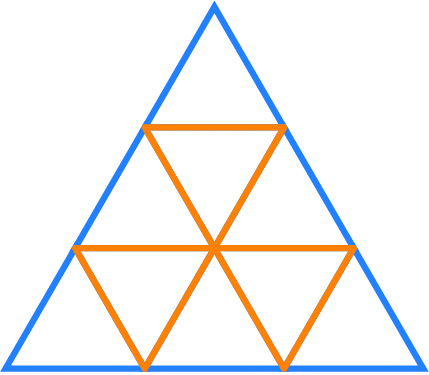
\includegraphics[width=0.18\textwidth]{Hinh24_1}
		\caption{\color{red}{\fbox{\small Tổng toàn bộ : $\color{red}9 \!+\! 3\! +\! 1 \!=\! 13$}}}
		\vspace*{-10pt}
	\end{figure}
\end{multicols}
\begin{multicols}{2}
	\begin{table}[H]
		\setlength{\tabcolsep}{2pt}
		\renewcommand{\arraystretch}{1.3}
		\begin{tabular}{|c|c|c|c|}
			\hline
			Vị trí & {\color{timhieukhoahoc}{Lên}}  & {\color{duongvaotoanhoc}{Xuống}} & {\color{red}{Tổng}}\\
			\hline
			Kích thước $1$  & ${\color{timhieukhoahoc}{10}}$ &${\color{duongvaotoanhoc}{6}}$ & ${\color{red}{16}}$ \\
			\hline
			Kích thước $2$  & ${\color{timhieukhoahoc}{6}}$ & ${\color{duongvaotoanhoc}{1}}$ &  ${\color{red}{7}}$ \\
			\hline
			Kích thước $3$  & ${\color{timhieukhoahoc}{3}}$ & ${\color{duongvaotoanhoc}{0}}$ & ${\color{red}{3}}$\\
			\hline
			Kích thước $4$  & ${\color{timhieukhoahoc}{1}}$ & ${\color{duongvaotoanhoc}{0}}$ & ${\color{red}{1}}$\\
			\hline
		\end{tabular}
		%		\caption{Bảng $1$.}
	\end{table}
	\begin{figure}[H]
		\vspace*{5pt}
		\centering
		\captionsetup{labelformat= empty, justification=centering}
		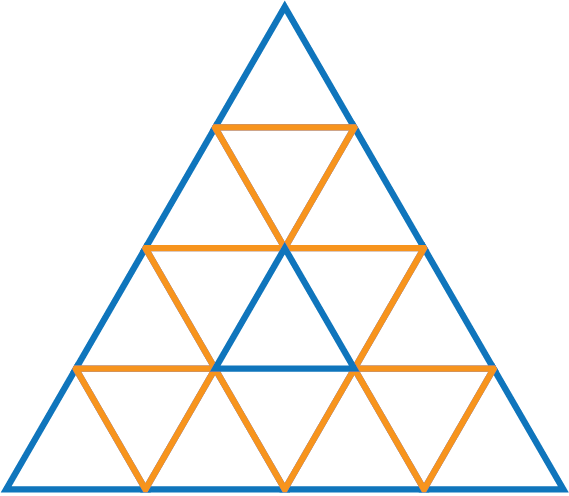
\includegraphics[width=0.235\textwidth]{Hinh25_1}
		\caption{\color{red}{\fbox{\small Tổng toàn bộ:$\color{red}16 \!+\! 7 \!+\! 3 \!+\! 1 \!=\! 27$}}}
		\vspace*{-10pt}
	\end{figure}
\end{multicols}
Từ bảng liệt kê trên, các bạn đã đoán được quy luật của số tam giác hướng lên và hướng xuống chưa? Chúng ta cùng xem lại qua  Hình $19$ với tam giác có cạnh kích thước $4$ nhé.
\vskip 0.1cm
$\bullet$Số tam giác ``hướng lên", liệt kê theo kích thước giảm dần tạo thành dãy có quy luật sau.
\begin{center}
	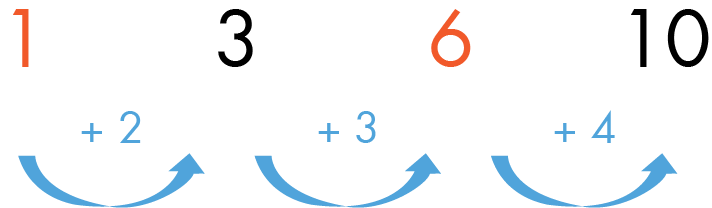
\includegraphics[width=0.3\textwidth]{QuyLuat}
\end{center}	
Nếu liệt kê theo thứ tự {\bf\color{toancuabi} tăng dần về kích thước} tạo thành dãy có quy luật dưới đây.
\begin{align*}
	(1+2+3+4), {\color{duongvaotoanhoc}{(1+2+3)}}, (1+2), {\color{duongvaotoanhoc}{1}}
\end{align*}
Số tam giác “hướng xuống”, liệt kê theo kích thước tăng dần, chính là số tam giác ``hướng lên" có thứ tự {\color{duongvaotoanhoc}{chẵn}} trong dãy trên.
\begin{align*}
	{\color{duongvaotoanhoc}{6}	\qquad \qquad	1 }
\end{align*}
Như vậy số tam giác trong Hình $19$ là: ${\color{timhieukhoahoc}{(1+3+6+10)}} + {\color{duongvaotoanhoc}{(1+6)}} = {\color{red}{27}}$.
\vskip 0.1cm
Với quy luật vừa tìm được này, chúng ta cùng đếm xem có bao nhiêu tam giác trong hình tam giác với kích thước cạnh là $5$ nhé.
Ta lập bảng số tam giác ``hướng lên" và ``hướng xuống" như sau.
	\begin{table}[H]
	\vspace*{-5pt}
	\centering
	\captionsetup{labelformat= empty, justification=centering}
	\setlength{\tabcolsep}{5pt}
	\renewcommand{\arraystretch}{1.3}
	\begin{tabular}{|c|c|c|c|}
		\hline
		Vị trí & {\color{timhieukhoahoc}{Lên}}  & {\color{duongvaotoanhoc}{Xuống}} & {\color{red}{Tổng}}\\
		\hline
		Kích thước $1$ & ${\color{timhieukhoahoc}{15}}$ & ${\color{duongvaotoanhoc}{10}}$ &${\color{red}{25}}$\\
		\hline
		Kích thước $2$ & ${\color{timhieukhoahoc}{10}}$ & ${\color{duongvaotoanhoc}{3}}$ & ${\color{red}{13}}$\\
		\hline
		Kích thước $3$ & ${\color{timhieukhoahoc}{6}}$ & ${\color{duongvaotoanhoc}{0}}$ & ${\color{red}{6}}$\\
		\hline
		Kích thước $4$ & ${\color{timhieukhoahoc}{3}}$ & ${\color{duongvaotoanhoc}{0}}$ & ${\color{red}{3}}$\\
		\hline
		Kích thước $5$ & ${\color{timhieukhoahoc}{1}}$ & ${\color{duongvaotoanhoc}{0}}$ & ${\color{red}{1}}$ \\
		\hline
	\end{tabular}
	\caption{\color{red}{\fbox{\small Tổng toàn bộ: $\color{red}25 + 13 + 6 + 3 + 1 = 48$}}}
\end{table}
Đến bây giờ, các bạn đã tìm ra ``câu thần chú" cho bài toán đếm hình này chưa? Hơi khó hơn một chút nhỉ? Chúng ta cùng phát biểu nhé.
\vskip 0.1cm
{\bf\color{toancuabi} Quy tắc $\pmb{4.}$} \textit{Số tam giác tạo ra từ một tam giác với cạnh kích thước $n$ có họa tiết kiểu tam giác bằng tổng số tam giác ``hướng lên" và tam giác ``hướng xuống", trong đó dãy các tam giác ``hướng lên" và ``hướng xuống" được liệt kê dưới đây.
	\vskip 0.1cm
	$\bullet$ Số tam giác ``hướng lên" với kích thước cạnh lần lượt là $1, 2,\ldots, n-1, n$ tạo thành dãy số có quy luật sau.
	\begin{align*}
		&(1\!+\!2\!+\!\ldots\!+\!n), (1\!+\!2\!+\!\ldots\!+\! n\!-\!1), \ldots,(1\!+\!2), 1 
	\end{align*}
	$\bullet$ Số tam giác ``hướng xuống" với kích thước lần lượt là $1, 2,\ldots$ tạo thành dãy số sau. Dãy này lấy từ các số có thứ tự chẵn trong dãy chỉ số tam giác ``hướng lên".}
\begin{align*}
	(1 \!+\! 2 \!+\! \ldots \!+\! n\!-\!1), (1 \!+\! 2 \!+\! \ldots \!+\! n\!-\!3),\ldots
\end{align*}
Các bạn nhỏ hãy sử dụng ``câu thần chú" ở trên để làm bài tập sau nhé. 
\vskip 0.1cm
{\bf\color{toancuabi} Bài tập $\pmb{4.}$} Hãy đếm xem có bao nhiêu tam giác có được từ tam giác với hoa văn kiểu tam giác ở trên, có cạnh kích thước cạnh là $6$.
\vskip 0.1cm
Các bạn nhỏ thân mến, vậy là chúng ta đã cùng nhau hoàn thành được $4$ nhiệm vụ trên chặng đường “đếm tam giác”. Những “câu thần chú” đưa ra thật là thú vị phải không? Các bạn hãy ghi nhớ để khi cần đem ra dùng nhé. Đây không phải đã là tất cả các nhiệm vụ trên chặng đường “đếm tam giác”. Các bạn có thể sẽ gặp những nhiệm vụ mới trên chặng đường này hoặc gặp những nhiệm vụ nào đó trên chặng đường khác. Tuy nhiên, bất cứ khi gặp nhiệm vụ nào, hãy nhớ về cách chúng ta vừa làm cùng nhau. Hãy xuất phát từ những hình có kích thước (số lượng) nhỏ, quan sát, nhận xét và rút ra quy luật. Tất nhiên là ngồi làm và mày mò để rút ra quy luật sẽ là mất thời gian rồi, nhưng đây là những “câu thần chú” vô cùng hiệu nghiệm, giúp chúng ta những lúc cần chỉ việc hô “úm ba la” là kết quả sẽ hiện ra. Một điều điều quan trọng hơn nữa đó là: Việc chúng ta tư duy tìm ra những “câu thần chú” như thế này sẽ rèn cho chúng ta “bản lĩnh” hơn, từ đó dễ dàng hoàn thành những nhiệm vụ đặt ra trên con đường học toán.